\documentclass[12pt, a4paper, openany]{report}

\usepackage[left=3cm,top=3cm, bottom=3cm, right=4cm]{geometry}

\usepackage{secdot} % Dots in Section Numbers
\usepackage[utf8]{inputenc}
\usepackage[T1]{fontenc}
\usepackage[ngerman]{babel}
\usepackage{graphicx}
\graphicspath{ {images/} }

\usepackage{soul}

\usepackage{fancyhdr}
\usepackage[textwidth=90, backgroundcolor=blue]{todonotes}
\usepackage{hyperref}

\usepackage{titlesec}
\titleformat{\chapter}[hang]{\Huge\bfseries}{}{0pt}{\Huge\bfseries}
\newcommand\frontmatter{ \cleardoublepage \pagenumbering{roman}}
\newcommand\mainmatter{ \cleardoublepage \pagenumbering{arabic}}
\newcommand\backmatter{ \if@openright \cleardoublepage \else \clearpage \fi }

\usepackage[autostyle]{csquotes}
\usepackage[
    backend=biber,
    style=alphabetic,
    sortlocale=de_DE,
    natbib=true,
    url=false,
    doi=true,
    eprint=false
    ]{biblatex}
\addbibresource{literatur.bib}

\usepackage{xparse}
\DeclareDocumentCommand \ATcite{m}{\citeauthor{#1}, \emph{\citefield{#1}{shorttitle}}}
\DeclareDocumentCommand \footATCite{ o o m } {%
  \IfNoValueTF {#2}{%
         \IfNoValueTF {#2}%
            {\footnote{\ATcite{#3}.}}%
            {\footnote{#1 \ATcite{#3}.}}}%
         {%
         \IfNoValueTF {#1}%
            {\footnote{\ATcite{#3}, S. #2.}}%
            {\footnote{#1 \ATcite{#3}, S. #2.}}}}

\DeclareDocumentCommand \qq{m}{\glqq #1\grqq}
\DeclareDocumentCommand \q{m}{\glq #1\glq}

\pagestyle{fancy}
\fancyhf{}
\lhead{Jan van Dick}
\chead{\glqq Zweite Natur und Befreiung\grqq}
\rhead{\thepage}

\title{
    {Zwischen Kritik und Affirmation}\\ 
    {\large- Zweite Natur und Befreiung bei Hegel und Nietzsche}\\
    {\large(Between Critique and Affirmation - Second Nation and Liberation in the Philosophies of Hegel and Nietzsche)}\\
    {\bigskip}
    {\large Goethe Universität Frankfurt am Main}\\
    {\bigskip}    
    {\bigskip}    
    {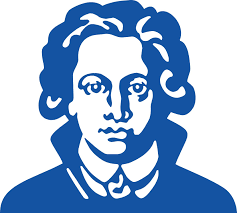
\includegraphics{logo.png}}\\
    {\bigskip}    
    {Sommersemester 2020}\\
}
\author{
    {Jan van Dick}\\
    {6081227}
}
\date{\today}

\begin{document}

\maketitle
\frontmatter


\chapter*{Abstrakt} \todo[noline]{Ist das Abstrakt so sinnvoll?}
Friedrich Nietzsches These vom Tode Gottes aus \textit{Die Fröhliche Wissenschaft}, dass \glqq wir\grqq{} ihn getötet haben, ist mehr als bloße Negativität. 
Müsste der Mensch nicht selbst Gott werden, um ihn getötet zu haben?.\footfullcite[Vgl.][481]{nietzsche_morgenrote_1999} 
Und der Mensch ist Gott dadurch geworden, dass er ihn \textit{geschaffen} hat, dadurch nur konnte er ihn töten. 
In dem Tod Gottes, liegt, dass Gott selbst vom Menschen gesetzt, dass er Schein ist, der sich gegen ihn verselbstständigte.
Gott ist somit geistiges Produkt des Menschen, in dem der Geist selbst wieder zur Natur sich verkehrte.
Der Tod Gottes ist die Befreiung daraus.
Der \glqq Tolle Mensch\grqq{} erklärt aber zugleich, dass nur die wenigsten von dieser Tat wissen. 
Für die Einen ist der Tod Gottes, eine untergegangene Sonne, die Befreiung also wieder eine In-Natur-Verkehrtheit.
Nur für uns \glqq geborene Räthselrather\grqq, die den Tod Gottes im vollen Umfang begreifen, ist er ein \glqq neues offenes Meer\grqq\footATCite[][573]{nietzsche_morgenrote_1999}.
Ist nun der Tod Gottes, die Befreiung aus der von ihm gesetzten Natur, das unbekannte, neue, offene, noch nie so offen gewesene Meer, oder ist er der Beginn des Wieder-in-Natur-Verkehrt-Seins, wie Christoph Menke es in der Analyse Hegels Begriffs der zweiten Natur beschreibt?\footfullcite[Vgl.][144]{menke_autonomie_2018}\\
Befreiung steht also zwischen Kritik (wieder-in-Natur-Verkehrtheit) und Affirmation (Einheit von Setzen und Sein).
Während Menke (und Hegel) Befreiung aus der zweiten Natur, nicht ohne eine neu hervorgebrachte zweite Natur, in welcher der Geist wieder in Natur verfällt lesen, erörtere ich die Frage, ob es in dem Motiv des \glqq neuen offenen Meeres\grqq{} und der \glqq geborenen Räthselrather\grqq{} bei Nietzsche, eine Befreiung aus der fortwährenden In-Natur-Verkehrtheit geben kann.
Es ist die Frage nach einer dritten Befreiung neben der Befreiung aus der 1. und der 2. Natur. 
Die Antwort dazu wird sich in der Arbeit als Ergebnis des Unterschiedes der \glqq Erkennenden\grqq{} bei Nietzsche geben:
Zwar kann Befreiung aus der Natur nicht ohne Setzen einer zweiten Natur geschehen, aber die Befreiung, die sich in dem Bewusstsein ihrer eigenen Kritik vollzieht, ist zugleich über ihrer eigene Befreiung hinaus.
Die dritte Befreiung ist damit allerdings keine Befreiung aus der Befreiung.
Befreiung bleibt notwendig: der Mensch kann Freiheit nicht \textit{haben}, er muss sie immer wieder selbst hervorbringen.


\tableofcontents

\mainmatter

\chapter{Einleitung}
So, wie Friedrich Nietzsche in dem Aphorismus vom \glqq Tollen Menschen\grqq{} in \textit{Die fröhliche Wissenschaft} die These vom Tode Gottes entfaltet, enthält sie weit mehr als die bloße Negation Gottes;
in ihr steckt eine dialektische Konzeption der Begriffe (zweite) Natur und Befreiung.\footfullcite[Vgl.][481]{nietzsche_morgenrote_1999}
Diese beiden Begriffe möchte ich aus der Sicht Nietzsches, sowie der von Christoph Menke rekonstruierten Perspektive Hegels untersuchen.
Beide Begriffe entfalten sich in ihrem Doppelcharakter: zweite Natur als Kritik und Affirmation, Befreiung als Macht und Ohnmacht des Geistes.
In der zweiten Natur schlägt Setzen in Sein um; hierin liegt zum Einen die Verwirklichung des Geistes (Affirmation), zum Anderen die In-Natur-Verkehrtheit, der Tod des Geistes durch den Geist (Kritik).\footfullcite[Vgl.][145]{menke_autonomie_2018}
Ebenso verhält es sich mit dem Begriff der Befreiung: 
sie ist 1. die \textit{Macht} des Geistes neues Hervorzubringen und die scheinbare Notwendigkeit des Bestehenden zu durchbrechen, 
2. aber die \textit{Ohnmacht} des Geistes, da die Befreiung nie abgeschlossen ist; die Macht der Befreiung ist die Schaffung einer \glqq neuen\grqq{} zweiten Natur, aus der der Geist sich befreite und nun erneut befreien muss.\footATCite[Vgl.][80]{menke_autonomie_2018}\\
Doch während in Hegels Deutung der Geist in der Befreiung aus der zweiten Natur, auf Grund der Endlichkeit des menschlichen Geistes, wieder in Natur verfällt, scheint bei Nietzsche in der Metapher des neuen, offenen Meeres, die Perspektive die ewige Wiederholung der In-Natur-Verkehrtheit zu überwinden, gegeben zu sein.
Zugleich betonen sowohl Hegel, als auch Nietzsche Freiheit als nicht-gegeben: 
Freiheit wird bei beiden so gedacht, dass man sie \glqq nicht nur hat, sondern auch beständig  noch erwirbt und erwerben muss\grqq\footATCite[][637]{nietzsche_morgenrote_1999}. 
Freiheit ist die Befreiung aus der jeweiligen Unfreiheit.\footfullcite[Vgl][227]{adorno_negative_dialektik_2003}\todo[noline]{Eingehen auf Geist = sich von Natur unterscheiden?} \\ 
Die Dialektik zwischen Freiheit und Notwendigkeit, Geist und Mechanismus, Endlichkeit und Unendlichkeit des Geistes, ist demnach Gegenstand meiner Arbeit. 
Die Leitfrage der Arbeit also: \textit{gibt es in Nietzsches Philosophie eine Möglichkeit der Überwindung der Notwendig-in-Natur-Verkehrtheit des Geistes?}\\
Aus der Position des oben erwähnten \glqq Tollen Menschen\grqq{} liegt es nahe, diese Möglichkeit in dem \textit{Vollzug} der Befreiung zu denken. 
Genauer: in einer Form des Bewusstseins in der Tätigkeit der Befreiung; 
eine Befreiung, die sich im Bewusstsein ihrer eigenen Kritik vollzieht.
Zugleich, muss aber der Schein selbst, \glqq mich fühlen lassen, dass hier Schein [...] und nichts mehr ist\grqq\footATCite[][417.]{nietzsche_morgenrote_1999}.
Zu Fragen demnach, ob dieses Bewusst-Werden eine Arbeit des einzelnen Individuums ist, oder ob es aus der Struktur des Allgemeinen, aus der zweiten Natur, dem Schein selbst, hervorgehen kann.\\

Nietzsche Aussage über den Tod Gottes bedeutet nach der Form-Seite die Überwindung der vom Menschen gesetzten zweiten Natur (Gott), der inhaltlichen Seite nach aber, dass der Mensch Gott nicht mehr nötig hat und die Bestimmung des Gesetzes sich aus dem Menschen selbst entwickelt. \todo[noline]{Muss Autonomie in die Einelitung hineingenommen werden?}
In diesem Sinne ist Kants Philosophie der Versuch einer Begründung der Moral aus der reinen praktischen Vernunft und dadurch eine Begründung der Moral die nicht von Gott abhängt. 
Ob für Nietzsche Kants Philosophie der Ursprung des Todes Gottes ist, oder bereits der Beginn des offenen Meeres, lasse ich dahingestellt, argumentiere aber selbst, dass er beides ist.
Um also den Begriff der zweiten Natur zu erarbeiten, werde ich kurz auf Kants Autonomieformel eingehen, da hier der Versuch Gesetz und Freiheit zusammen zudenken seinen Ursprung nimmt. 
Der Begriff der zweiten Natur ergibt sich dann aus Hegels Kritik an Kants Autonomiebegriff:
versucht Kant zwar mit dem kategorischen Imperativ aus dem Paradox der Autonomie zu entkommen, argumentiert Hegel, dass er sich hier in der Inhaltslosigkeit des Gesetzes wiederholt.
Hegels Ausweg besteht darin Freiheit sozial zu verstehen. 
Aus dieser Perspektive werde ich Hegels Begriff der Sittlichkeit als soziale Teilhabe entwickeln.
Doch auch hier wird sich das Paradox der Autonomie in der Begriff der Gewohnheit wiederholen.
Aus der erneuten Wiederholung des Paradox werde ich Hegels Begriff der Befreiung entwickeln.
Darin ergibt sich, wie oben angegeben, die Grenze des von Menke erarbeiteten Begriffs der Befreiung:
Macht und Ohnmacht der Befreiung: Freiheit und Unfreiheit bleiben untrennbar miteinander verbunden.
Durch die Hinzunahme Nietzsches, soll versucht werden über diese Grenze hinauszugehen.\\

Zunächst soll der Begriff der zweiten Natur aus der Perspektive Hegels erläutert werden. 
In einem \hyperref[abschnitt_1]{ersten Schritt} soll demnach der Hegelsche Begriff der zweiten Natur anhand von folgendem Zitat Menkes rekonstruiert werden:
\begin{itemize}
    \item[] Die Gewohnheit als zweite Natur [ist] geistig oder frei [...], insofern sie ein Ausdruck des Wollens (oder ein Setzen) ist, und [...] mechanisch oder unfrei [...], weil sie, einmal gesetzt, selbstständig und unbewusst wirkend ist.\footATCite[][145]{menke_autonomie_2018}
\end{itemize}
Die Struktur des ersten Teils ergibt sich aus den zu klärenden Begriffen. 
Zuerst soll der Begriff der Gewohnheit aus der Sittlichkeit, als Schritt über den \glqq bloß moralischen Standpunkt[]\grqq\footfullcite[][§ 135, S.139]{hegel_grundlinien_2017} hinaus, erläutert werden (a). 
Daraus ergibt sich der Begriff des \glqq geistigen Mechanismus\grqq, in welchem die Gewohnheit sich als \glqq geistig oder frei\grqq{} und \glqq mechanisch oder unfrei\grqq{} ergibt.\footATCite[][145]{menke_autonomie_2018} (b).
Schließlich soll der Begriff der zweiten Natur aus Hegels Perspektive, seinen Abschluss finden in der Dialektik zwischen endlichem und unendlichem Geist und dem Doppelcharakter der zweiten Natur als Kritik und Affirmation (c).\\
In einem \hyperref[abschnitt_2]{zweiten Schritt} soll gezeigt werden, dass bei Nietzsche ein ähnlicher Begriff der zweiten Natur aufgezeigt werden kann.\footnote{Ich halte diesen Schritt unter anderem des deshalb für sinnvoll, weil er rechtfertigt, warum ich meine, mit Nietzsche überhaupt über Menkes Begriff der Befreiung hinausgehen zu können.}
\todo[noline]{Generell mehr Begründung, wieso Nietzsche?}
Dabei soll bereits auf die Beantwortung der Leitfrage vorbereitet werden.
Zunächst soll der Begriff der zweiten Natur anhand von Nietzsches Begriff des \textit{Scheins} erläutert werden (a).
Die Befreiung aus dem (sog.) Schein wird darauffolgend in der Unterscheidung des Schauspielers und der Rolle aufgegriffen (b). 
Abschließend sollen beide Begriffe nochmals in dem Absatz über den tollen Menschen analysiert und zusammengebracht werden (c).
In der Darlegung Nietzsches Position wird der Begriff \glqq Bewusstsein der Scheinhaftigkeit\grqq{} bereits eine wichtige Rolle einnehmen und dient der späteren Beantwortung der Leitfrage.\\
Im \hyperref[abschnitt_3]{dritten Abschnitt} soll die Befreiung aus der zweiten Natur erläutert werden, da diese, im Vergleich zur Befreiung aus der ersten Natur bei Hegel und Menke, und letztendlich auch bei Nietzsche, uneindeutig bleibt.
Wie Befreiung aus der zweiten Natur überhaupt möglich ist und wie diese sich konkret vollzieht, ist notwendig, um zu diskutieren wie über diese hinausgegangen werden kann.\\
Im vierten und \hyperref[abschnitt_4]{letzten Schritt} soll es abschließend zu einer Diskussion und Beantwortung der Leitfrage kommen. 


\chapter{Hauptteil}
\todo[noline]{Hier besser Einschub über Geist $\leftrightarrow$ Natur?.}
Die folgende Diskussion um Befreiung und zweite Natur wird ihren Ausgangspunkt in der Kritik der Autonomie finden, aus dem ich zu Hegels Begriff der Sittlichkeit kommen werde. 
Es mag merkwürdig anmuten, dass ich gerade mit der Kritik an der Autonomie beginne und hier, als Ausgangspunkt dieser Kritik, den Begriff einer positiven Bestimmung der Freiheit hinterfrage,
wo die Leitfrage meiner Arbeit doch letztendlich auf einen positiven Begriff der Freiheit hinausläuft, auf eine Befreiung, die die Unfreiheit hinter sich lassen kann.
Dennoch und trotzdem, liegt meiner Arbeit, wie den beiden Autoren, zu jeder Zeit Adornos Bestimmung der Freiheit als Befreiung aus der jeweiligen Unfreiheit zu Grunde.
Der Versuch eines Hinausgehen, über den Begriff der Befreiung hinaus oder durch ihn hindurch, hin zu einem positiven Begriff von Freiheit, ist ohne die Kritik an dem positiven Begriff der Freiheit, zum Scheitern verurteilt.
\todo[noline]{Was ist genau mit positiver Freiheitbegriff gemeint?}
Meine Vorstellung eines positiv bestimmten Freiheitsbegriffs, oder die Befreiung über die Befreiung hinaus, ist die Befreiung, die sich als Unfreiheit weiß; die Befreiung also, die positiv bestimmt ist, aber nur in der Negation realisiert werden kann. 

\section{Zweite Natur bei Hegel}\label{abschnitt_1}
Der Begriff der Freiheit kann nicht als reine Unbestimmtheit oder bloße Abstraktion von allem verstanden werden.\footATCite[Vgl.][38, §5]{hegel_grundlinien_2017} 
Sondern die Freiheit kann nur gefunden werden, wo eine Bestimmung des Selbst vorhanden ist.
Allerdings muss diese Bestimmung selbst die Form der Freiheit besitzen. 
Thomas Khurana drückt dies so aus, dass das Subjekt einer Bestimmung bedarf, die dem Ich einen konkreten Inhalt gibt und (diese Bestimmung) selbst die Form des Ich erhält\footATCite[Vgl.][285]{khurana_freiheit_2017}. 
Freiheit des Willens ist also eben das: sich \glqq als \textit{bestimmt}, \textit{beschränkt} zu setzen und bei sich, d.i. in seiner \textit{Identität} mit sich und Allgemeinheit zu bleiben.\grqq\footATCite[][40, §7]{hegel_grundlinien_2017}
Ein Versuch Freiheit als diese Einheit von Freiheit und Bestimmung zu verstehen ist der Begriff der Autonomie. 
Der Begriff der Autonomie, wie Kant ihn erarbeitet, nimmt schließlich eine positiven Realisation der Freiheit an.
Freiheit jedoch so zu verstehen, dass man sie beständig noch erwerben muss\footATCite[Vgl.][636]{nietzsche_morgenrote_1999}, bedeutet Freiheit als Befreiung zu verstehen. 
Freiheit also als einen Akt zu verstehen, der noch (oder immer wieder) geschehen muss.
Damit heißt Freiheit als Befreiung zu denken, wie Hegel, Menke, Adorno und (wie ich argumentieren werden) auch Nietzsche es tun, Freiheit negative zu verstehen und aus der Negation heraus zu begreifen.
Immanuel Kant versucht in der Bestimmung der Freiheit als Selbstgesetzgebung, Freiheit so zu bestimmen, dass dieser Akt der Negation verschwindet. 
Dieser Versuch ist bei Kant zugleich der Versuch das Paradox der Autonomie aufzulösen. 
Hegels Kritik der Autonomie versucht hingegen aufzuzeigen, dass sich dieses Paradox in der Selbstgesetzgebung auch bei Kant erneut wiederholt.
Ich möchte zunächst anhand von Hegels Kritik der Autonomie den Begriff der Sittlichkeit erarbeiten.
Aus diesem komme ich zur Gewohnheit, welche
\begin{itemize}
    \item[] [...] als zweite Natur geistig oder frei ist, insofern sie ein Ausdruck des Wollens (oder ein Setzen) ist, und mechanisch oder unfrei ist, weil sie, einmal gesetzt, selbstständig und unbewusst wirkend ist.\footATCite[][145]{menke_autonomie_2018}
\end{itemize}
Hieran zeigt sich, dass in der Sittlichkeit das Paradox der Autonomie erneut auftritt. 
Anhand des Zitates, werde ich die sich hier entfaltende Dialektik von Geist und Mechanismus, sowie Kritik und Affirmation beschreiben und daraus die Begriffe zweite Natur und Befreiung erarbeiten und an ihnen den Ausweg aus dem Paradox skizzieren.

\subsection{(a) Autonomie und Sittlichkeit}
\todo[noline]{Alles aus Gott ist tot herleiten?}
Der Tod Gottes bei Nietzsche hat, wie in der Einleitung bereits erwähnt, nicht bloß die Bedeutung der Befreiung aus der zweiten Natur, sondern ist ebenso eine Reflexion auf die Umwälzung innerhalb der (Moral-)Philosophie seines und des vorangegangenen Jahrhunderts. 
Waren doch die Gesetze der Moral durch Gott bestimmt und die Freiheit als die Befolgung dieser Gottesgesetze, so entzieht die Überwindung Gottes diese Gesetze der außer dem Menschen liegende Macht. 
Der Tod Gottes beginnt deshalb auch dort, wo die Moral nicht mehr bloß durch Gott bestimmt ist. 
Der Begriff der Autonomie versucht nun zweierlei: 
er versucht die Bestimmung der Moral von Gott zu lösen und in den Menschen zurückzuführen, ohne jedoch den Schritt hinter Gott zurückzutreten und Freiheit wieder durch blindes Bestimmt-Sein durch die Natur, die sinnlichen Triebfedern, zu sehen. 

\subsubsection{Kant und das Paradox der Autonomie}
Autonomie bedeutet zunächst Gesetz und Freiheit nicht als einander gegenübergestellt, sondern als sich gegenseitig ergänzend und bestimmend zu betrachten: 
nicht in dem blinden Folgen meiner sinnlichen Triebe, sondern in dem Handeln nach dem Gesetzt bin ich frei. 
Und ein Gesetzt ist nur dasjenige, unter dessen Befolgung ich frei bin. 
Autonom zu sein bedeutet also meinem selbst gegebenem Gesetzt zu folgen. 
Autonomie bedeutet, dass freies Wollen und verpflichtendes Sollen in eins fallen.\footATCite[Vgl.][19]{menke_autonomie_2018}\\
Die Selbstgesetzgebung ist ebenso der Ort, an dem das Paradox der Autonomie auftritt: 
die Selbstgesetzgebung, in der die Autonomie einsetzen soll, ist selbst nur als heteronom zu denken: 
entweder folgt die Selbstgesetzgebung aus einem anderen, äußeren Gesetz (äußere Heteronomie) oder beruht auf der freien Willkür des Subjekts (innere Autonomie).\footATCite[Vgl.][20]{menke_autonomie_2018}\\
Indem Kant die Autonomieformel beinahe wörtlich wiederholt, aber den Fokus von \textit{Selbst}Gesetzgebung zu \textit{eigener} Gesetzgebung verlegt, beschreibt er das Gesetz nicht als für das Subjekt bereits vorhanden, welches dieses nur auswählt, sondern als Gesetz des Subjekts selbst.
Diese eigenen Gesetze hätten nach Kant gleichwohl allgemeinen Charakter.\footfullcite[Vgl.][65]{kant_kritik_2014} 
Das Subjekt wird also als Urheber des Gesetzes gesehen, doch wie kann dieses eigene Gesetz allgemein gültige Notwendigkeit haben, wie kann es als objektives Gesetz der Vernunft gelten?
Die Antwort auf diese Frage liegt in dem kategorischen Imperativ: \glqq \textit{handle nur nach derjenigen Maxime, durch die du zugleich wollen kannst, dass sie ein allgemeines Gesetz werde}\grqq\footATCite[][51. Im Original gesperrt gedruckt]{kant_kritik_2014}.
Selbstgesetzgebung bedeutet bei Kant also nicht, dass das Subjekt sich ein bestehendes Gesetz gibt, sondern \glqq seinen Antrieben die \textit{Form} des Gesetzes zu geben\grqq\footATCite[][24]{menke_autonomie_2018}.
Autonomie bedeutet bei Kant demnach durch die Wahl der Maxime diese zum allgemeinen Gesetz zu machen. 
Das Gesetz ist also wesentlich durch die Freiheit bestimmt.
Ebenso auch die Freiheit durch dass Gesetz, denn wie alles Gesetzen unterliegt, müsse dies auch für den freien Willen gelten.
Und die Kausalität des freien Willen ist \glqq die Eigenschaft des Willens, sich selbst ein Gesetz zu sein\grqq\footATCite[][81]{kant_kritik_2014}.\\

Damit ist bei Kant das erreicht, was ich oben als das Ziel des Begriffs der Autonomie aufzeigte: 
das normative Gesetz ist zurück bei dem Menschen und obliegt nicht einer Macht außerhalb des Menschen (Gott), zugleich wird Freiheit nicht verstanden als blindes Unterliegen der sinnlichen Triebfedern. 
Freiheit ist bei Kant negativ bestimmt als das Frei-Sein von sinnlichen Antrieben, aber zugleich in dem Begriff der Selbstgesetzgebung positiv realisiert. 
Der Mensch \textit{ist} also frei. 
Freiheit bedarf keiner Negation mehr.\footATCite[Vgl.][53]{menke_autonomie_2018}
Wie eingangs behauptet verstehen Hegel und Nietzsche Freiheit aber gerade so, dass sie noch werden muss. 
Kant gelangte zur positiven Realisation der Freiheit mit seinem Begriff der Selbstgesetzgebung. 
In diesem wiederholt sich allerdings nach Hegel das Paradox der Autonomie. Der kategorische Imperativ ist nur durch die \textit{Form} bestimmt und bleibt selbst inhaltsleer.
Die Maxime muss die Form des allgemeinen Gesetzes haben, welches aber selbst keine Bedingungen hat:
es \glqq bleibt damit nur die abstrakte Allgemeinheit [...] oder das Abstrakte \textit{Positive}, dass Bestimmungslose zu ihrer Bestimmung\grqq{} und Kants Autonomieformel verkommt zum \glqq leeren Formalismus\grqq.\footATCite[][139, §135]{hegel_grundlinien_2017}
Das Paradox besteht darin, dass die Freiheit nur in der Inhaltslosigkeit zu denken ist, der Inhalt kann aber nur von außen hinzukommen, liegt also nicht mehr innerhalb der Selbstgesetzgebung und der Traum der positiven Realisation der Freiheit verpufft.
\todo[noline]{Umformulieren?}

\subsubsection{Hegels Auswegen in der Sittlichkeit}
Worin genau besteht nun Hegels Ausweg aus dem Paradox?
Die Kritik Hegels, an Kants Begriff der Autonomie, hat seinen Grund auch in dem, was ich weiter oben als Notwendigkeit der Verknüpfung von Abstraktion vom Inhalt (also bestimmungslosigkeit) und Bestimmung (sich einen Inhalt geben), nannte. 
Freiheit kann letztendlich nur dort herrschen, wo dieser Doppelcharakter verwirklicht ist.\footnote{Wie wir im Folgenden und letztendlich in dem Begriff der Befreiung sehen werden, ist das so auch dies nicht ganz richtig.}
Dieser Doppelcharakter ist der, welcher sich letztendlich in der Sittlichkeit ausdrückt, welche Hegel als \qq{die Idee der Freiheit, als das lebendige Gute, das in dem Selbstbewusstsein sein Wissen, Wollen und durch dessen \textit{Handeln} seine Wirklichkeit [...] hat}\footATCite[][161, §142. Hervorhebung von mir]{hegel_grundlinien_2017}.
Indem Hegel hier den Begriff der Handlung einführt, bekommt der Begriff der Autonomie eine neue Wendung. 
Das Gute hat in dem Selbstbewusstsein sein Wissen und Wollen, aber in seiner \emph{Handlung} seine Wirklichkeit. \todo[noline]{Was beutet an der Stelle Wissen, und was das \qq{lebendige} Gute}
Und in dieser Wirklichkeit erst ist es \emph{lebendig}.
Dass die Idee der Freiheit als das \emph{lebendige} Gute aufgefasst wird, könnte wieder als Gegenthese zum leeren Formalismus bei Kant gelesen werden:
nur in dem die Individuen handelnd das Gute verwirklichen \emph{lebt} es, nur so ist die Idee der Freiheit verwirklicht und das ist die Sittlichkeit.
Diese Handlung ist nun selbstverständlich nicht beliebige Handlung, sondern die Handlung innerhalb einer bestimmten (sittlichen) Praxis.\footnote{Bzw. die Praxis \emph{ist} sittlich, gerade indem Subjekte handelnd an ihr Teilnehmen.}
Damit ist der Begriff der Sittlichkeit wesentlich sozial bestimmt.
Menke beschreibt dies als das soziales Teilnehmen an einer Praxis. \footATCite[Vgl.][28 ff]{menke_autonomie_2018}
Von der Seite der Teilnahme gedacht ist so zu verstehen, inwiefern das Gute zu seine, Inhalt kommt: im Gegensatz nämlich zum \qq{abstrakten Guten} (bei Kant), ist das \qq{objektiv Sittliche [...] durch die Subjektivität \emph{konkrete} Substanz}\footATCite[][161, §144]{hegel_grundlinien_2017}.
Das objektiv Sittliche, oder das Gesetz, ist damit \emph{das Eigene} des Subjekts, in dem es durch dessen handeln sich konstituiert. 
Dies Gesetz hat, nach Hegel, \qq{eine [...]  unendlich festere Autorität und Macht, als das Sein der Natur}\footATCite[][164, §146]{hegel_grundlinien_2017}
Dies kann man sich, um einen ersten Bogen zu Nietzsche zu schlagen, an dem Beispiel Gottes verdeutlichen: 
indem der Mensch Gott durch sein Handeln (beten, zur Kirche gehen, etc.) schafft, schafft er ihn als ein Gesetz, welches die der Natur ersetzt. 
Wie ja wirklich die Macht der Natur durch Gott aufgehoben und dieser für z.B. Naturkatastrophen verantwortlich gemacht wird.
Zugleich gibt Gott (mit den Zehn Geboten) den Mensch seine ersten Gesetze.
\footnote{%
    Auf das Motiv Gottes, als das Setzen einer ersten zweiten Natur, werde ich mich noch einige Male beziehen. 
    Ich lasse hier grundsätzlich die mir ansonsten sehr einleuchtende Spezifizierung Khuranas aus, in welcher er drei Stufen unterscheidet, in denen das Hervorgehen aus und das Setzen der Natur sich wiederholt: Anthropologie, Phänomenologie und Sittlichkeit.
    Erst die dritte dieser Stufen stellt die Sittlichkeit, als \qq{der zur \emph{vorhandenen Welt} und \emph{zur Natur des Selbstbewusstseins gewordene Begriff der Freiheit}} (\ATcite{hegel_grundlinien_2017}, S. 161) dar und nur auf diese beziehe ich mich hauptsächllich, während ich die anderen Stufen in meinen Ausführungen größtenteils auslasse.
    Khurana unterscheidet von der Sittlichkeit 1. die Anthropologie, in der der Geist mittels der Gewohnheit aus seiner noch in Natur versenkten Form sich befreit und 2. die Phänomenologie, in welcher der Geist seiner selbst bewusst wird. 
    (\ATcite{khurana_freiheit_2017}, S. 394 - S. 397)
    Die Schaffung Gottes, ist demnach eher in der ersten oder zweiten Stufe zu suchen, als in der Sittlichkeit. 
    Um den Rahmen der Arbeit allerdings nicht zu sprengen, verweise ich hier nur auf diese Unterscheidungen und benutze Gott als ein allgemeines Beispiel, denn was damit auf gezeigt wird trifft auf alle Stufen in gleicher Weise zu. 
    Es sollte nur vermieden werden Gott als ein Beispiel von Sittlichkeit zu sehen. 
    Dies ist meiner ansich nach nicht der Fall.
}\\

In der sozialen Teilnahme an einer Praxis, und das ist das entscheidende, konstruiert das Subjekt jedoch nicht nur das Gesetz, als ein dann ihm fremdes, sondern es konstituiert damit auch sich selbst. 
Damit sei zweierlei gesagt: 1. sind die Gesetze, oder ist das Gesetz, welches er in einer bestimmten Praxis konstituiert, dem Subjekt nicht fremd und 2. haben die von dem Subjekt konstituierten Gesetz wiederum konstituierenden Einfluss auf das Subjekt. 
Hegel drückt dies aus, indem er schreibt, die Gesetzte sind \qq{dem Subjekt nicht ein Fremdes, sondern es gibt das \emph{Zeugnis des Geistes} von ihnen als von \emph{seinem eigenen Wesen}}\footATCite[][162, §147]{hegel_grundlinien_2017}.
Die Gesetze stehen dem Subjekt 1. nicht Fremd gegenüber, da sie durch seine eigene Handlung gesetzt sind und aus dem selben Grund konstituieren sie 2. das Subjekt, da es seine eigenen autonomen Handlungen sind;
es wird konstituiert \qq{durch eben die Gesetze, die die Praxis konstituieren}\footATCite[][30]{menke_autonomie_2018}, und das sind seine eigenen.
Sittlichkeit und soziale Teilhabe so verstanden, lösen somit das Paradox der Autonomie auf, denn die Gesetze sind hier sowohl inhaltlich bestimmt, als auch autonom gesetzt.
Bevor ich nun dazu übergehe zu beschreiben, wie sich in der Sittlichkeit das Paradox dennoch wiederholt, sei an dieser Stelle schon darauf verwiesen, dass Hegel den Moment, in welchem \qq{das Sittliche die wirkliche Lebendigkeit des Selbstbewußtseins ist}, als \qq{Verhältnis-lose Identität}\footATCite[][163, §147]{hegel_grundlinien_2017} beschreibt. 
Von diesem Punkt aus ist es schwer sich eine Transformation des Gegebenen vorzustellen.
Wie diese Transformation, oder die Befreiung in der Sittlichkeit zu denken ist, werde ich im \hyperref[abschnitt_3]{dritten Abschnitt} diskutieren.

\subsubsection{Die Wiederholung des Paradox: Zweite Natur}
Wie oben bereits in der Analogie zu Gott erwähnt, schafft der Mensch in der Sittlichkeit sich Gesetze, die zwar 1. das Paradox der Autonomie aufheben, d.h. sie sind eigene, inhaltlich bestimmte und zugleich Wesens-Konstituierend Gesetze, aber sie werden 2. zu einer Macht, die noch die Macht der Natur überbietet in der Autorität für den Menschen.
D.h. das Schaffen (oder Setzen) von Gott, gibt den Menschen die Moral, aber versklavt ihn zugleich einer neuen, inneren Notwendigkeit: \qq{das Sittliche [erscheint] als eine \emph{zweite Natur}}.
\footnote{\ATcite{hegel_grundlinien_2017}, S. 166, §151.
Wie hier der Begriff des \qq{Erscheinens} zu verstehen ist, ist mir etwas unschlüssig. 
Als Lesart schlage ich vor, dass Hegel so verstanden werden muss, dass Sittlichkeit als zweite \emph{Natur} und nicht als \emph{zweite} Natur erscheint. 
Und sie \emph{erscheint}, weil es \emph{zweite}, vom Menschen gesetzte Natur ist, darum, denke ich, spricht Hegel von \emph{Erscheinen} nicht von \emph{Sein}.
Würde sie übrigens, damit greife ich auf \hyperref[abschnitt_2]{den zweiten Abschnitt} vor, als \emph{zweite} Natur erscheinen, wäre in gewissermaßen bereits erfüllt, was Nietzsche fordert: dass der Schein mich spüren lässt, dass er Schein und nichts weiter ist. \footATCite[Vlg.][416, §54]{nietzsche_morgenrote_1999}.}

Im Gegensatz zu Kant, bei dem die moralisch verstandene Befreiung des Mensch den Bruch mit der äußeren Notwendigkeit (Triebe, natürliche Determination etc.) bedeutet, kann bei Hegel die Befreiung nur darin liegen, die natürliche Determination, die äußere Notwendigkeit, die Macht der ersten Natur zu ersetzen, durch eine geistig, selbst hervorgebrachte, \qq{selbstgemachte[] Notwendigkeit}\footATCite[196, § 194]{hegel_grundlinien_2017}.
Darum schreibt Hegel, die verwirklichte Freiheit ist aus dem Menschen hervorgebracht, als eine zweite Natur.\footATCite[Vlg.][34, §4]{hegel_grundlinien_2017}
Dies bedeutet aber zugleich, dass der Mensch, nur frei sein kann, indem er selbst eine neue, sei es Natur, oder innere Notwendigkeit, aber eine Form der Verknüpfung schafft, die \emph{nicht geistig}, sondern \emph{natürlich} ist. 
Menke beschreibt dies als die \qq{\emph{eigene} natürliche Verfassung des Geistes}, in der aber \qq{das Werden seiner Autonomie}\footATCite[][40. Hervorhebung von mir]{menke_autonomie_2018} erst entstehen kann.
Die Hervorbringung einer eigenen natürlichen Verfassung, einer eigenen Gewohnheit erscheint also hier als Grundbedingung und Ergebnis von Sittlichkeit und Befreiung.
Nietzsche erkennt das und schreibt daher, dass es nach dem Tod Gottes \qq{noch Jahrtausende lang Höhlen geben [wird], in denen man seinen Schatten zeigt. - Und wir - wir müssen auch noch seinen Schatten besiegen!}\footATCite[][467, §108]{nietzsche_morgenrote_1999}
Das ist die eine Seite, die Nietzsche beschreibt, die andere ist aber, die Gefahr des Sonnenuntergangs, die Gefahr, dass es \emph{keine} neue Form der Verknüpfung geben wird.
\footnote{Diese Sonnenfinsternis als eine mögliche Folge, beschreibt Nietzsche als Folge von Zerstörung und Zerfallen und Unbestimmtheit, welcher der wieder freie Horizont gegenübersteht. 
Die Schädlichkeit also die absolute Abstraktion, die \qq{Zertrümmerung aller bestehenden gesellschaftlichen Ordnung}\footATCite[][39]{hegel_grundlinien_2017}, also die absolute Unbestimmtheit zur Bestimmung zu nehmen, wie wir schon in der Einleitung zu Hegels Freiheitsbegriff gesehen haben, ist auch bei Nietzsche problematisch und hängt eng zusammen mit dem Problem der zweiten Natur.
Wie Sonnenfinsternis, Schatten und offenes Meer genauer verstanden werden müssen, werde ich im \hyperref[abschnitt_2]{zweiten Abschnitt} genauer erläutern.}
Es muss die vom Geist selbst hervorgebrachte, selbstgemachte Notwendigkeit, die \emph{zweite} Natur geben (die Schatten), von der wir uns dann erneut befreien müssen (wir müssen auch sie noch töten).
Und damit bedeutet Befreiung nicht nur die Befreiung aus der ersten, sondern ebenso die Befreiung aus der zweiten Natur. 

In diesem Sinn ist auch zu verstehen, was es für Hegel heißt als Freiheit \qq{Reflexion des Geistigen in sich, seiner Unterscheidung von dem Natürlichen und seinem Reflex auf dieses}\footATCite[][197]{hegel_grundlinien_2017} zu verstehen: 
es bedeutet, dass Freiheit (und Geist) wesentlich das ausmacht sich \emph{immer wieder} von der Natur zu unterscheiden, sich permanent aus dieser zu befreien, sei es von der Natur, als erste Natur, oder von seiner eigenen natürlichen Verfassung.
Wir haben also die in sozialen Praktiken geistig produzierte zweite Natur, einerseits selbst als das Mittel der Befreiung von der Natur zu verstehen, zugleich aber als das wodurch sich die In-Natur-Verkehrtheit \emph{im Geist} wiederholt.\footATCite[Vgl.][41]{menke_autonomie_2018}
In diesem Sinne tritt hier das Paradox der Autonomie in der Sittlichkeit als Dialektik und Wechselwirkung zwischen Befreiung und zweiter Natur auf.
Diese innere Dialektik der Befreiung und der zweiten Natur werde ich im Folgenden mit Menke als die Dialektik von Geist und Mechanismus beschreiben.

\subsection{(b) Dialektik von Geist und Mechanismus}

\subsection{(c) Dialektik von Kritik und Affirmation}

\section{Zweite Natur bei Nietzsche}\label{abschnitt_2}

\subsection{(a) Was bedeutet Schein?}

\subsection{(b) Der Schauspieler und die Rolle}
\qq{Der Geist will sich befreien, als die Natur aus sich herausbildend}\footATCite[][393]{khurana_freiheit_2017}. 
Hier haben wir also genau das Verhältnis der Rolle: der Mensch setzt die Rolle als seine Natur. 
Die Rolle, die Geistig war, geistig geschaffen ist, \emph{wird} zur Natur. 
Dies ist also die eine Seite der Befreiung. 
Die zweite ist, der Schauspieler, der sich aus der Natur, der Rolle, die selbst nur zweite Natur, also Schein ist, befreit und stattdessen Kunst und Schein setzt. 
Aber mit dem entscheidenden Unterschied, dass dem Schauspieler seine Rolle nicht selbst wieder als Natur erscheint, der Schauspieler produziert etwas, das mich wissen lässt, dass hier Schein, Geistertanz und nichts weiter ist. 
Das ist der zu suchende Ausweg, wenn man sich die Frage nach der ewigen Wiederholung der Befreiung stellt.

\subsection{Exkurs: Nietzsche - Natur und Antisemitismus}
\todo[noline]{Dieser Abschnitt muss allgemein überarbeitet werden. Die Frage ist, ob das Thema Antisemitismus nicht den Rahmen sprengt an dieser Stelle. Auch als Exkurs}
In dem vorherigen Abschnitt stellt Nietzsche den Schauspieler und die Rolle gegenüber. 
In dieser Gegenüberstellung tritt noch eine dritte \glqq Persönlichkeit\grqq{} auf: der Baummeister. 
Außerdem vergleicht, bzw. identifiziert Nietzsche den Schauspieler mit den Juden und den Frauen (\glqq Welcher gute Schauspieler ist heute nicht Jude\grqq\footATCite[][608]{nietzsche_morgenrote_1999}).
Diese Gegenüberstellungen und Identifizierungen möchte ich zum Anlass nehmen auf einen weiteren Punkt einzugehen, der mit den Gegenstand der Arbeit nicht unmittelbar, aber mittelbar zusammenhängt. 
Für Nietzsche ist, wie eingangs beschrieben, Schein nicht der Gegensatz zu dem Wesen, zur Natur, sondern Schein, oder Kunst, ist das Wirkende und Lebende selber.\footATCite[Vgl.][416]{nietzsche_morgenrote_1999} 
Diese Stelle, und andere vorher erwähnte Stellen, legen nahe, dass es für Nietzsche überhaupt gar nicht etwas, wie erste Natur gibt, sondern, dass alles Schein, zweite, vom Menschen geschaffene Natur ist.
Zugleich ist bei Nietzsche häufig eine Unterscheidung zwischen den \glqq Vornehmen\grqq{} und den \glqq Gemeinen\grqq{} aufzufinden, in dem diese Unterschiede von Nietzsche scheinbar als natürliche Unterschiede aufgezeigt werden. 
\todo[noline]{Zitate finden: Genealogie d. Moral/ Jenseits von G u. B.}
Wie stellt sich an diesen Stellen also die Frage nach der (ersten) Natur?
Wenn der Schauspieler eigentlich der von Nietzsche affirmierte Charakter ist (so jedenfalls die Annahme), wie verhält sich es sich mit dem Baummeister, der als dieser Natürliche, Vornehme gesehen werden kann? 
Der Baumeister zeichnet sich aus durch Kraft und Mut und dadurch die Gesellschaft zu bauen, für die \glqq wir\grqq{} nicht mehr das richtige Material sind etc. 
Er steht im Gegensatz zu dem Schauspieler, dem Künstler, dem Wechselhaften, Ungebundenen, Heimatlosen. 
Er scheint eben das Natürliche zu verkörpern, er ist der, der \glqq von Natur aus\grqq{} so ist und darin die alten Werte aufbewahrt.\\
Diese Gegenüberstellung erscheint bei Nietzsche zunächst antisemitisch:
dem Schauspieler, den Frauen, den Juden wird der Baummeister, der ehrliche, mutige, beinahe mag man sagen \glqq deutsche\grqq{} Wesenszug entgegengestellt.
Das wir alle schon zu sehr Schauspieler geworden seinen oder der \glqq Amerikaner-Glaube\grqq\footATCite[][596]{nietzsche_morgenrote_1999} immer weiter nach Europa dringt, wirkt wie die völkische, oder zumindest konservative  Kritik an der jüdischen, wahlweise liberalen oder bolschewikischen Verschwörung.
Auf ähnliche Weise könnten hier Nietzsches Beschäftigungen mit dem \glqq Sklavenaufstand der Moral\grqq{} herangezogen werden, in welchen Nietzsche die Schwachen dafür kritisiert aus einem Gefühl der Unterlegenheit heraus den Starken ihre Moral aufzuzwingen. 
Die Sklavenmoral steht bei Nietzsche im schroffen Gegensatz zu der Moral \glqq alle[r] vornehme[n] Moral[, die] aus einem triumphierenden Ja zu sich selbst herauswächst\grqq\footfullcite[][S. 10?]{nietzsche_jenseits_2014} 
An dieser Stelle wird jedoch ersichtlich, dass Nietzsches Identifikation des Schauspielers mit den Juden und Frauen gerade aus der entgegengesetzten Richtung stammt:
die scheinbare Kritik an den Juden, sie seien \glqq jenes Volk der Anpassungskunst par excellence\grqq\footATCite[][609]{nietzsche_morgenrote_1999} mutet antisemitisch, muss aber aus dem selben Blickwinkel gedeutet werden, aus dem heraus Nietzsche die Sklavenmoral kritisiert:
dann wird deutlich, dass Nietzsches Kritik sich nicht gegen die Schauspieler wendet, sondern viel mehr gegen jene, die aus einem Gefühl der eigenen Unterlegenheit die Macht dieser aus der Perspektive der Sklavenmoral heraus kritisieren. 
Anders gesagt: aus der Perspektive Nietzsches Kritik am Ressentiment gehören nicht die Juden und die Frauen und die Schauspieler zum Ressentiment, sondern gerade die Antisemiten, die Gender-Kritiker, die Baumeister. 
\todo[noline]{Letzte Argumentation nicht ganz schlüssig}
Auch an den Stellen also, an den Nietzsche scheinbar das Natürliche, oder Angeborene, hervorhebt, zeigt sich, dass sich dieses nur durch das \glqq Ja-sagen zu sich selber\grqq{} durch das Sich-selbst-Hervorbringen, das Spielen und mit der eigenen \glqq Natur\grqq{} entwickelt, dass nur diejenigen vornehm sind, die ihre scheinbare Natur bespielen und wieder in Kunst aufgehen lassen.

\subsection{(c) Gott ist tot!}
\section{Was heißt Befreiung aus der zweiten Natur}\label{abschnitt_3}
\section{Das offene Meer?}\label{abschnitt_4}

\chapter{Fazit}

\backmatter

\printbibliography
\listoftodos
 
\end{document}
